\newpage
\section{Тестирование}
\subsection{Функциональное тестирование}
\begin{table}[!h]
    \caption{Функциональное тестирование}
    \begin{tabularx}{450pt}{|l|X|X|X|X|}
        \hline
        \textnumero & Название теста & Действия тестировщика & Ожидаемый результат & Прохождение теста\\
        \hline
        1 & Покупка недвижимости & Соглашается с предложением о покупке недвижимости & Недвижимость переходит во владение игрока. Со счёта игрока снимается стоимость недвижимость & Да\\
        \hline
        2 & Отказ от покупки недвижимости & Отказывается от предложения о покупке недвижимости & Недвижимость выставляется на аукцион & Да\\
        \hline
        3 & Залог недвижимости & Соглашается с предложением о залоге недвижимости & Недвижимость становится заложенной. Игроку перечисляются средства на счёт & Да\\
        \hline
        4 & Выкуп недвижимости & Соглашается с предложение о выкупе недвижимости & Недвижимость снова становится активной. Со счёта игрока снимается стоимость выкупа & Да\\
        \hline
    \end{tabularx}  
\end{table}
\subsection{Тестирование обучения нейронной сети}
Перед стартом обучения нейронной сети было протестировано преимущество противника, реализующего простейшую логику, перед противником, реализующим случайное поведение. Отношение побед оказалось 97 на 3 в пользу простой логики.

Нейронная сеть обучалась при параметрах:
\begin{spacing}{0.9}
\begin{enumerate}
    \item learning\_rate = 0.01
    \item gamma = 0.95
    \item размер памяти нейронной сети = 100
    \item размер обучающей выборки = 32
    \item epsilon = 1, epsilon\_min = 0.1, epsilon\_decay = 0.995
\end{enumerate}
\end{spacing}

\subsubsection*{Обучение нейронной сети в игре против случайного поведения противника}
\newpage
\begin{figure}[h!]
    \center{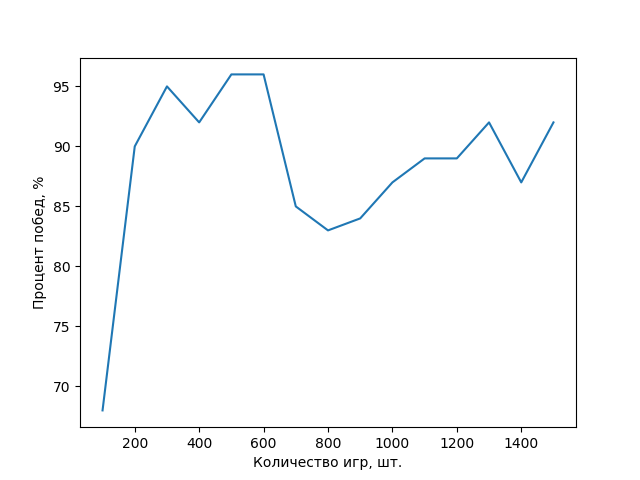
\includegraphics[scale=0.75]{rnn1.png}}
    \caption{Изменение процента побед в игре против случайного поведения противника}
\end{figure}
\begin{figure}[h!]
    \center{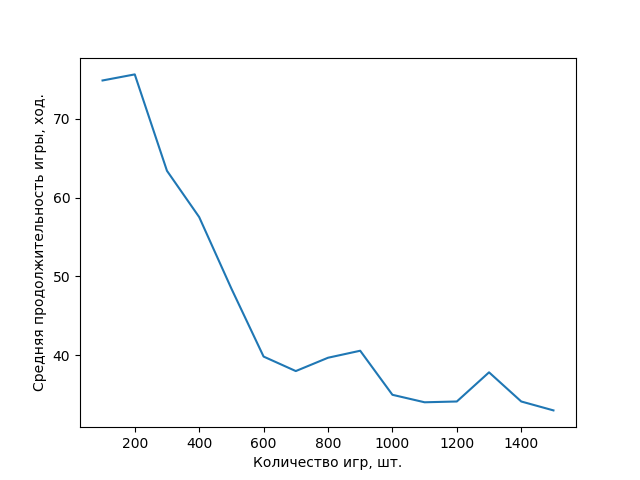
\includegraphics[scale=0.75]{rnn2.png}}
    \caption{Изменение средней продолжительности игры в игре против случайного поведения противника}
\end{figure}
\subsubsection*{Обучение нейронной сети против простого поведения противника}
\begin{figure}[h!]
    \center{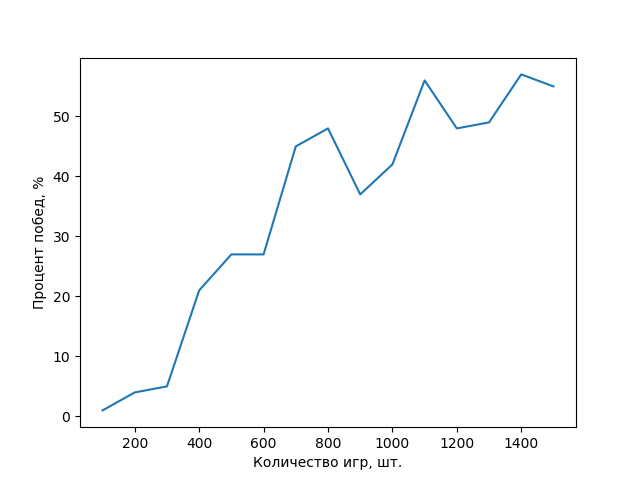
\includegraphics[scale=0.75]{snn1.png}}
    \caption{Изменение процента побед в игре против простого поведения противника}
\end{figure}
\begin{figure}[h!]
    \center{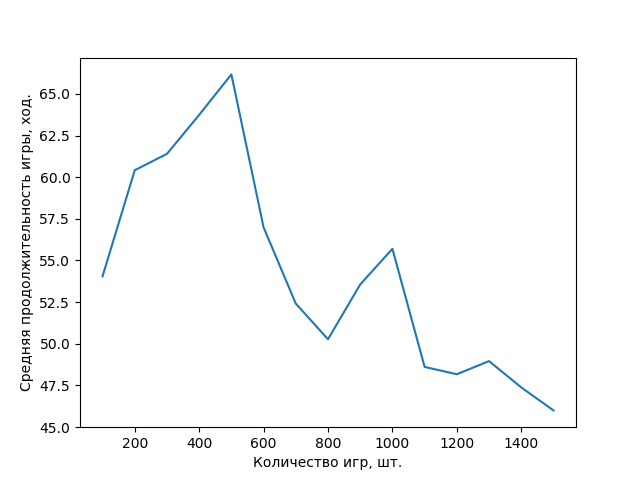
\includegraphics[scale=0.75]{snn2.png}}
    \caption{Изменение средней продолжительности игры в игре против простого поведения противника}
\end{figure}
\subsection*{Выводы}
\addcontentsline{toc}{subsection}{Выводы}
В ходе тестирования были проведены несколько экспериментов, которые обнаружили достоинства и недостатки алгоритма Q-обучения. 

Достоинства:
\begin{spacing}{0.9}
\begin{enumerate}
    \item Отсутствие необходимости формирования обучающей выборки перед началом обучения
    \item Возможность формирования стратегии игрока в функции награды
\end{enumerate}
\end{spacing}

Недостатки:
\begin{spacing}{0.9}
\begin{enumerate}
    \item Возможное переобучение
    \item Сложность формирования действий нейронной сети, подлежащих обучению
    \item Сложность определения функции награды
\end{enumerate}
\end{spacing}

Для улучшения процента побед предлагается:
\begin{spacing}{0.9}
\begin{enumerate}
    \item Изменение функции награды
    \item Улучшение алгоритма выбора совершенных действий нейронной сети, подлежащих обучению.
\end{enumerate}
\end{spacing}